\documentclass[12pt, a4paper]{article}
\usepackage[margin = 1in, top=1.3in]{geometry}
\usepackage[english]{babel}
\usepackage[utf8]{inputenc}
\usepackage{fancyhdr}
\usepackage{amsmath}
\usepackage{bm}
\usepackage{graphicx}
\graphicspath{{./images/}}
\usepackage[font=small,labelfont=bf]{caption}
 
\pagestyle{fancy}
\fancyhf{}
\rhead{\small{Niraj Mahajan \\ Raaghav Raaj}}
\lhead{CS-215 Assignment-4 : Question 3}
\rfoot{Page 3.\thepage}
 
\begin{document}
\section*{Question 3}
\subsection*{3.1 : Part A}
\hspace{1cm} For a given 2D dataset, we need to estimate a best fit linear relationship between the two random variables from which this dataset is drawn. We will use PCA for this. \\ 
Let $x_i$ and $y_i$ be the coordiates obtained in the $i^th$ draw, and let $\mathbf{X}$ be a matrix of two vectos, each corresponding to the x and y coordinates.\\ \\
The mean vector can be given by $\boldsymbol{\mu} =  
\begin{bmatrix}
\frac{\sum x_i}{n} &  \frac{\sum y_i}{n} 
\end{bmatrix}^T  = 
\begin{bmatrix}
\mu_x &  \mu_y 
\end{bmatrix}^T $ \\
The Covariance matrix can be given by $\mathbf{C} = \frac{1}{r-1}\mathbf{(X-\boldsymbol{\mu})^T(X-\boldsymbol{\mu})}$ \\ where, $r = no. \; of\; rows\; in\; \mathbf{X}$ \\ \\
Matrix $\mathbf{C}$ will have two eigenVectors. Let they be $\mathbf{V_1}$ and $\mathbf{V_2}$, with eigenvalues \\ $\lambda_1$ and $\lambda_2$ \\ 

The principle mode of variation will be along the eigenvector corresponding to the maximum eigenvalue. And hence this will be the most accurate approximation for a linear relation between the two Random Variables since the variation is maximum along the direction of the principle mode of variation. This also implies that the squared sum of distances of all data points will be minimum from a line passing through the sample mean, along this direction. Hence this will be the best fit line \\  \\
Hence, to derive the equation of the best fit line: \\
WLOG, let $\lambda_1 > \lambda_2$. Hence our principle mode of variation will be along the eigenvector $\mathbf{V_1} = \begin{bmatrix}
v^1_x &  v^1_y 
\end{bmatrix}^T $ (let) 

\begin{align*}
\frac{y-\mu_y}{x-\mu_x} &= \frac{v^1_y}{v^1_x}\\
y-\mu_y &= \frac{v^1_y}{v^1_x}.(x-\mu_x) \\
y &= \mu_y + \frac{v^1_y}{v^1_x}.(x-\mu_x)
\end{align*}

Thus we have derived an equation for the best fit plot using PCA!.

\subsection*{3.2 : Part B}
\noindent The plots for the first dataset along with a best fit plot showing the linear relationship between Y and X follows:

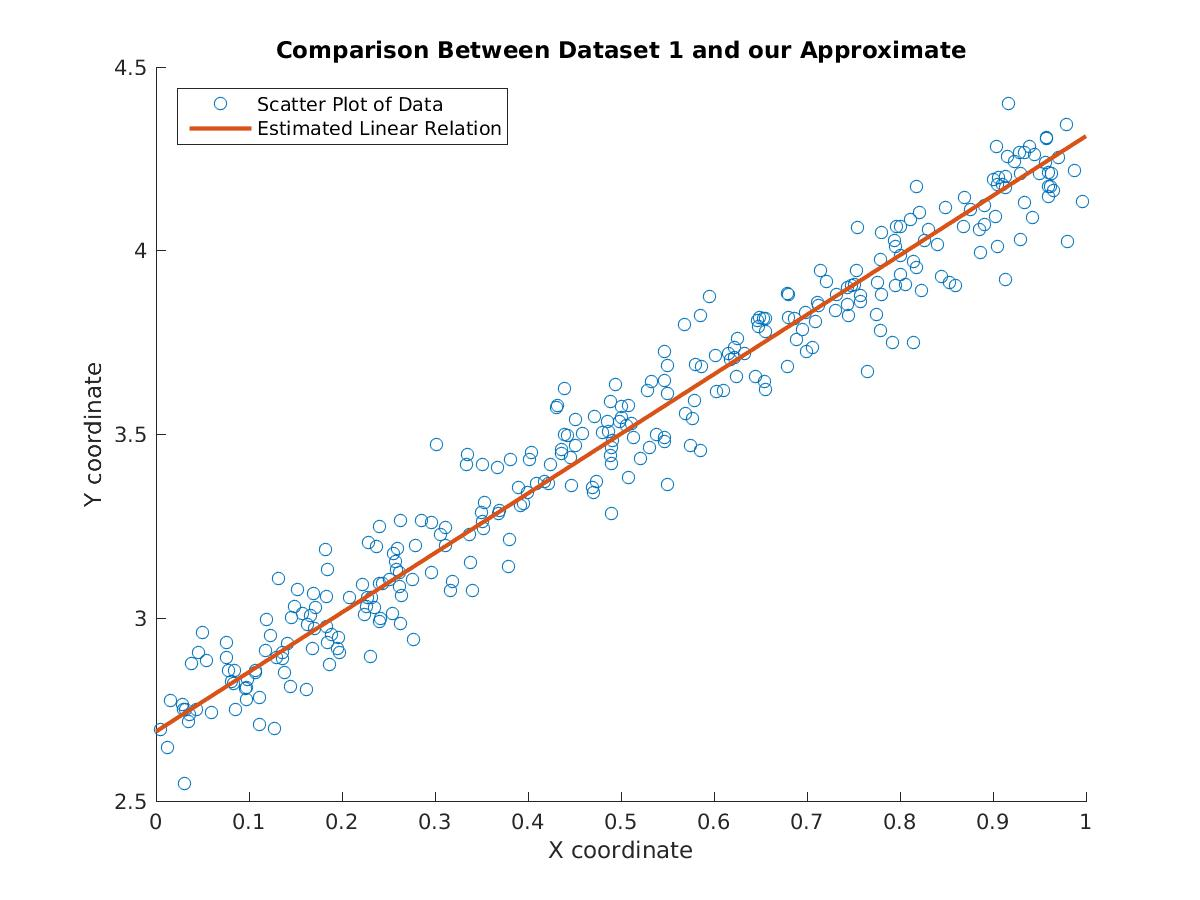
\includegraphics[width=\textwidth, height = 0.4\paperheight]{Dataset_1}

\subsection*{3.3 : Part C}
The same procedure was repeated for another Dataset. \\ 
\\ But in this case, the results were not very good. The second dataset was drawn from Random Variables where X, Y coordinates did not have a linear relationship between them. Hence fitting a straight line into this data is obviously a bad idea. 
\\ \\ Upon performing PCA, we got a best fit \lq straight line\rq \space through the data but this is not a good model. Instead of a linear model, perhaps a quadratic model could have given a better result.
\\ \\ \noindent The plots for the second dataset along with a best fit plot showing the linear relationship between Y and X follow: (PTO)
 
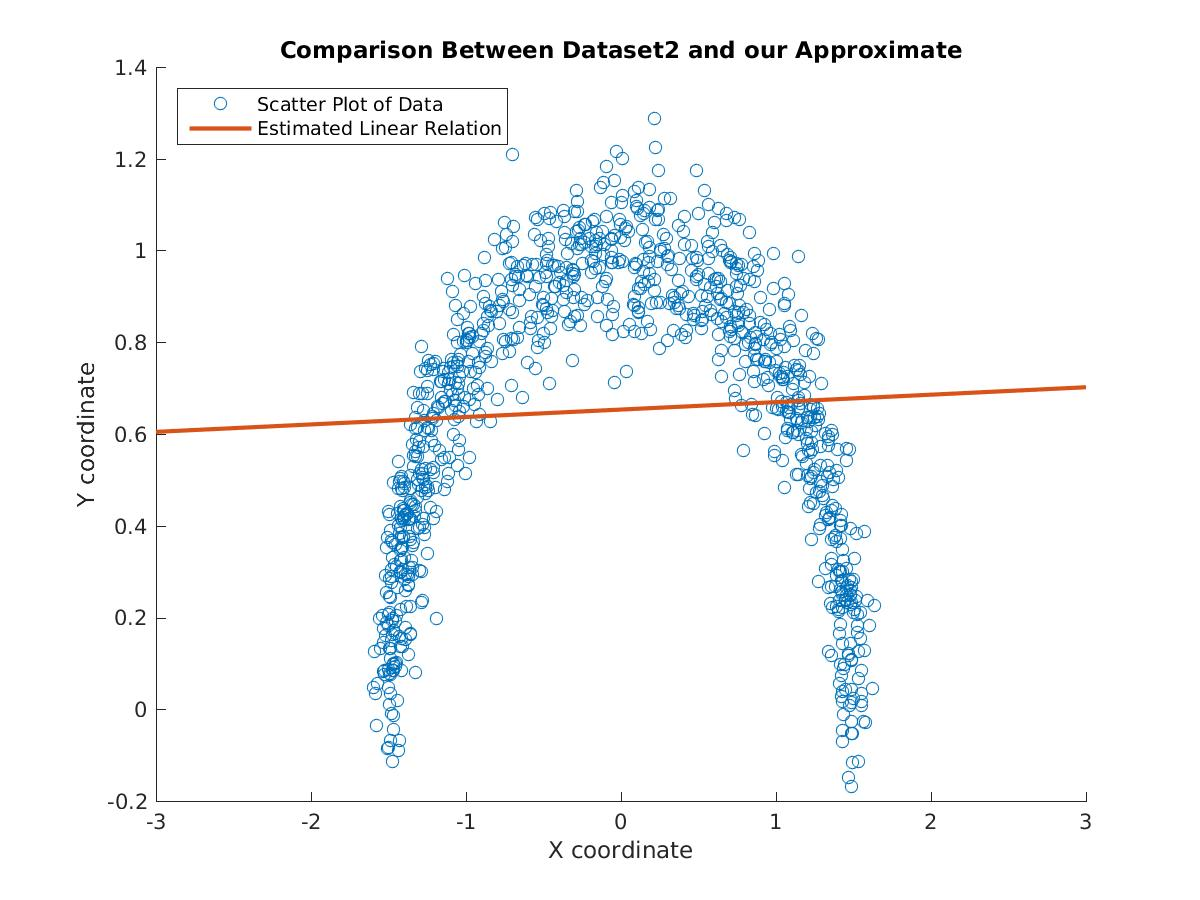
\includegraphics[width=\textwidth, height = 0.4\paperheight]{Dataset_2}
 
\subsection*{3.4 : Usage of Code}
The following are the instructions for the usage of the code:
\begin{itemize}
\item Load the code present in \lq submission/code/q3/q3.m \rq \space.
\item In the same directory are functions implemented like myMean, myCov which return the mean and covariance of appropriate matrices. Function myeigs will return the eigenvalues and corresponding eigenvectors in sorted order
\item Simply run the code in \lq q3.m \rq \space and this wil automatically create the required plots.
\item Lines 22, 45 (commented by default) hava a code to save jpg files of the respective plots. Comment/Uncomment these lines appropriately according to need.
\end{itemize}
 
 
\end{document}